\documentclass[conference]{IEEEtran}
%\IEEEoverridecommandlockouts
% The preceding line is only needed to identify funding in the first footnote. If that is unneeded, please comment it out.
\usepackage{cite}
\usepackage{amsmath,amssymb,amsfonts}
\usepackage{algorithmic}
\usepackage{graphicx}
\usepackage{textcomp}
\usepackage{xcolor}
\def\BibTeX{{\rm B\kern-.05em{\sc i\kern-.025em b}\kern-.08em
    T\kern-.1667em\lower.7ex\hbox{E}\kern-.125emX}}

\begin{document}

\title{ESE 2180 Project 2 Writeup}

\author{\IEEEauthorblockN{Chris Brusie}
\IEEEauthorblockA{\textit{Deptartment of Electrical Engineering} \\
\textit{Washington University in St. Louis}\\
St. Louis, United States \\
brusie@wustl.edu}
\and
\IEEEauthorblockN{Sebastian Theiler}
\IEEEauthorblockA{\textit{Deptartment of Electrical Engineering} \\
\textit{Washington University in St. Louis}\\
St. Louis, United States \\
s.k.theiler@wustl.edu}
\and
}

\maketitle


\section{Introduction}
Handwritten digit recognition is a fundamental problem in the field of computer vision and pattern recognition. The goal of this project was to classify images of hand-written digits, specifically determining if an image represents 0 or one of the digits 1-9. This was done through the use of least squares, a method of approximating solutions to overdetermined systems of equations. An exact solution to the system does not exist in our case, but an approximation can be made by taking advantage of projections and orthogonality. Then, we selected features to use for classification by identifying pixels that were active in at least 600 images. Our matrix was constructed from these feature vectors for each image and used with their corresponding labels to compute a learned set of features. This learned feature set was used to classify images, which resulted in relatively high accuracy, given the small training set. 

\section{Methods}
The methodology of this project can be broken into four main parts: identifying image features and constructing the matrices used for least squares, implementing the least squares classifier, classifying a training set of images using our learned features, and analyzing the effects of changing the feature vectors. 

\subsection{Identifying Image Features}
The first step of the project was to identify features of our training data set to be used in the classification problem. 

\subsection{Feature Transformation}
A feature transformation was implemented using a random matrix $R \in \mathbb{R}^{M \times M_0}$ with entries in $\{-1,1\}$ with equal probability, where $M_0$ was the original number of detected features (329) and $M$ describes the number of transformed features. The new feature vector for image $i$ was computed as:

$$z_i = \max\{Rx_i, 0\}$$

where $x_i$ is the original feature vector and the max operation is applied elementwise.

In code, this was performed as
\begin{verbatim}
def LS_classifier_artificial_features(
    M,
    R,
    x_train,
    y_train,
    pixels_to_consider,
    num_imgs
):
    x_train = np.array(x_train)
    x_data_flat = x_train.reshape(num_imgs, -1)
    X = x_data_flat[:, pixels_to_consider]
    A = np.maximum(R @ X.T, 0).T

    y = np.zeros((num_imgs, 10))
    for i, label in enumerate(y_train):
        y[i, label] = 1
    
    theta = np.zeros((M, 10))
    for digit in range(10):
        result = lsqr(A, y[:, digit])
        theta[:, digit] = result[0]

    return theta

\end{verbatim}

This transformation offers several advantages. First, the transformation allows us to explicitly control the feature space dimension through $M$. The mapping from $\mathbb{R}^{M_0}$ to $\mathbb{R}^M$ can either compress ($M < M_0$) or expand ($M > M_0$) the feature space. A compressed feature space may allow for faster computation, whereas an expanded feature space may allow the classifier to more easily find a separating hyperplane to classify digits. Additionally, the $\max{\cdot,0}$ operation introduces non-linearity into our otherwise linear classifier, which may allow the model to capture more complex decision boundaries.

\subsection{Experimentation with Feature Transformation}

Various values of $M$ were selected for experimentation: $M \in \{20, 50, 1000, 5000, 10000\}$, and error rate was calculated and recorded for each value of $M$ using the previously developed \texttt{test\_theta\_performance} function. This function was augmented to also accept $R$ as an input, which is then left-multiplied by $A^T$ before making predictions. The classifier was trained only on the first $2,000$ images of the MNIST dataset, as the increasing computational complexity of higher $M$ values made it infeasible to use a larger portion of the dataset. The relationship between $M$ and classification error followed an approximately exponential decay pattern as shown in Figure~\ref{fig:feature_transformation_error_rate}, where $M=20$ increased error rate to above 50\% while $M = 10,000$ decreased error rate to below 10\%, which is approximately half the original error rate of TODO\%. Increasing $M$ further may result in lower error rates; however, this comes at the cost of greatly increased computation time for diminishing improvements in quality.

\begin{figure}[htbp]
  \centerline{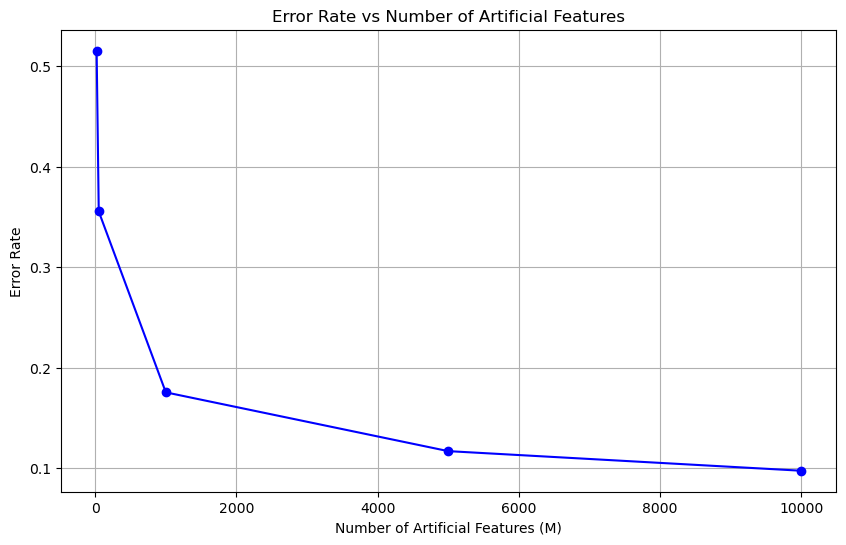
\includegraphics[scale=0.4]{figures/feature_transformation_error_rate.png}}
  \caption{Error Rate vs. Number of Artificial Features ($M$)}
  \label{fig:feature_transformation_error_rate}
\end{figure}  

\section{Results and Discussion}
The least-squares classifier can achieve reasonable performance on the MNIST dataset, particularly when using a sufficient number of training examples. Furthermore, multiple classifiers can be used to classify the dataset into individual digits---not just into 0 and non-zero digits while still maintaining a reasonable accuracy of TODO\%. This multi-class capability is noteworthy given the relative simplicity of the least-squares approach. The visualization of the learned parameters $\theta$ through heatmaps revealed interesting patterns for each digit classifier. These heatmaps effectively serve as "prototype" digits, where positive values (shown in warmer colors) indicate pixels that strongly contribute to identifying a particular digit, while negative values (cooler colors) represent pixels that suggest the absence of that digit. For instance, the classifier for digit "0" showed strong positive weights in a circular pattern, while the classifier for "1" emphasized a vertical pattern.

When reducing the training set size to just 100 images, we observed a significant degradation in performance, with the error rate increasing to approximately TODO\%. This deterioration can be attributed to the model not being exposed to an adequately broad range of training data and can therefore it cannot properly generalize to the variety of digits that appear in the MNIST training dataset. The least-squares classifier therefore has insufficient data to estimate the $\theta$ parameters reliably and is more susceptible to outliers in the dataset. In general, providing the model with more data will increase performance as it prevents the model from overfitting to a handful of images, creating a more robust model.

The transformation of the original features $x_i$ new features via $\max \{Rx_i, 0\}$ is interesting because $R$ allows us to explicitly control the feature dimension through $M$. This provides a systematic way to study the effect of the model's capacity on its performance. Aditionally, the combination of random projections with the max operation creates nonlinear features that measure the degree to which the input aligns with a random pattern (defined by a row of $R$), then zeros out negative alignments. This introduces a form of nonlinearity similar to modern neural networks' ReLU activations, allowing the classifier to capture more complex patterns than purely linear features would permit. However, there is a trade-off between model complexity and performance suggests that while increasing feature dimensionality generally improves accuracy, there exists an optimal point beyond which additional features provide minimal benefit.

\section{Conclusion}

This study demonstrates that least-squares classification for handwritten digit recognition can be effective despite the simplicity of the technique, achieving accuracy of TODO\%. It was found that training data volume significantly impacts model performance, with larger datasets leading to more robust classifiers. Reducing the training dataset to only 100 images resulted in a reduction in accuracy to TODO\%. Additionally, an important result was that random feature projection provides a powerful tool for controlling model complexity. Higher values of $M$ significantly increased the accuracy of the classifier, with $M = 5,000$ leading to a TODO\% accuracy; however, this came at the cost of significantly increased computational complexity, making it infeasible to train this expanded classifier on the full dataset, which, as previously discussed, has adverse effects on accuracy. Future work, such as exploring structured random projections or investigating how different nonlinearities after projection may allow least-squares to achieve even higher accuracy on MNIST digit classification.

\begin{thebibliography}{00}

\bibitem{spanishflu}
Cleveland clinic, 2021, “Spanish Flu: What Is It, Causes, Symptoms \& Pandemic,” Cleveland Clinic, Sep. 21, 2021. Available: https://my.clevelandclinic.org/health/diseases/21777-spanish-flu

\bibitem{b1} 
World Health Organization, 2021, "The True Death Toll of COVID-19: Estimating Global Excess Mortality," World Health Organization, May. Available: https://www.who.int/data/stories/the-true-death-toll-of-covid-19-estimating-global-excess-mortality

\bibitem{b2} 
United States Census Bureau, 2021, "Census Regions and Divisions of the United States," United States Census Bureau. Available: https://www.census.gov/geographies/reference-maps/2020/geo/division.html

\bibitem{walmart}
Walmart, 2024, “Mezorrison KN95 Face Masks, 50-Pack, Black,” Walmart. Available: https://www.walmart.com/ip/Mezorrison-KN95-Face-Masks-50-Pack-Black/518596184?classType=VARIANT

\end{thebibliography}

\end{document}
